\subsection{Memento (\textit{o Token})}
\label{memento}

\textbf{Scopo}: Comportamentale \\
\textbf{Raggio d'azione}: Oggetti

\paragraph{Definizione} Il pattern Memento permette di catturare ed esternale lo stato interno di un oggetto, senza violare l'incapsulamenteo, in modo tale che, in un secondo momento, sia possibile ripristinare un oggetto nello stato esportato.

È opportuno usare il pattern Memento quando:
\begin{itemize}
    \item si deve memorizzare un'istantanea (totale o parziale) dello stato di un oggetto, così da poterla ripristinare in un secondo tempo;
    \item si vogliono proteggere dettagli implementativi che violerebbero l'incapsulamento.
\end{itemize}

\begin{figure}[H]
    \centering
    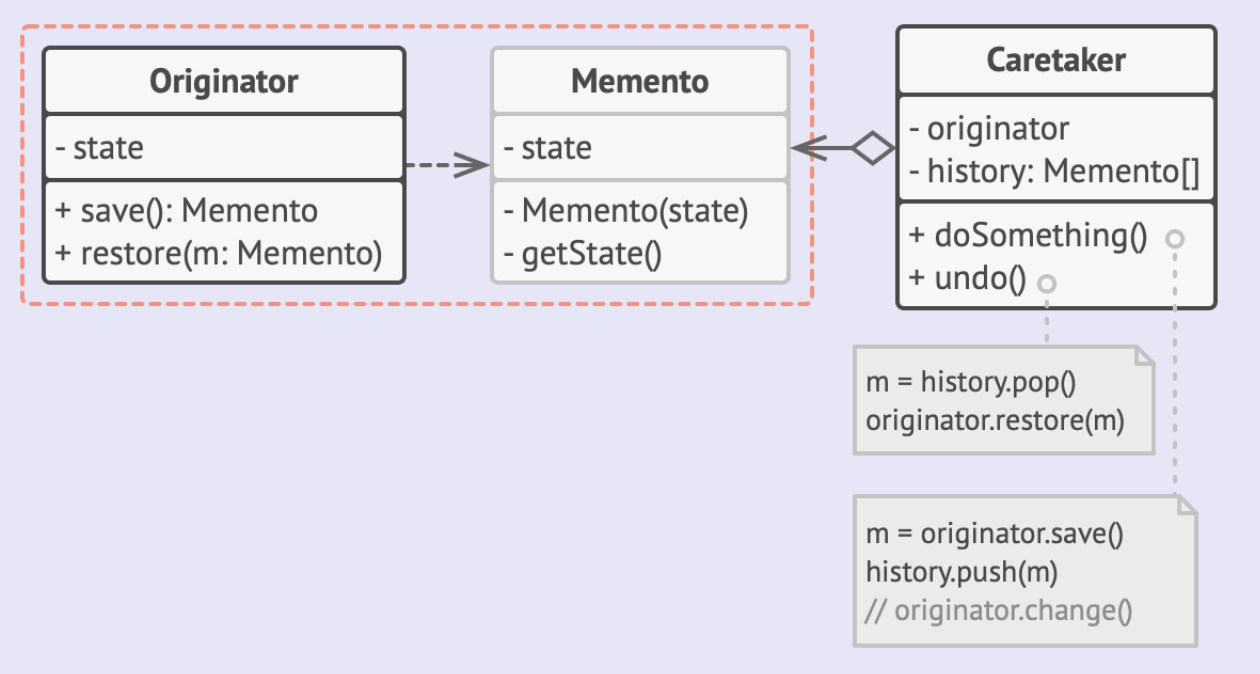
\includegraphics[width=1\linewidth]{assets/pattern/memento/memento-struttura.png}
    \caption{Struttura del pattern}
\end{figure}

\paragraph{Struttura e Conseguenze} Il pattern è composto da
\begin{itemize}
    \item \textbf{Memento}: memorizza lo stato interno dell’oggetto Originator, non permette l’accesso alla sua struttura dati se non all’Originator, presentando così due interfacce.
    \item \textbf{Originator} Crea un Memento contenente un’istantanea del proprio stato interno corrente. Usa un Memento per ripristinare il proprio stato interno tramite l’interfaccia estesa di Memento, con la quale è possibile accedere a tutti i dati necessari. Idealmente solo l’Originator che ha prodotto il Memento ha il permesso di accedere allo stato interno del Memento. 
    \item \textbf{Caretaker} È responsabile di memorizzare i Memento. Non invoca operazioni né esamina i contenuti di un Memento, vede un’interfaccia ridotta di Memento e può solo passare il Memento ad altri oggetti.
\end{itemize}

In altre implementazioni, la classe Memento è annidata all'interno di Originator. Ciò consente all'Originator di accedere ai campi e ai metodi del Memento, anche se sono dichiarati privati. D'altra parte, il Caretaker ha un accesso molto limitato ai campi e ai metodi del ricordo, il che gli consente di archiviare i ricordi in uno Stack ma di non manometterne lo stato.

\begin{figure}[H]
    \centering
    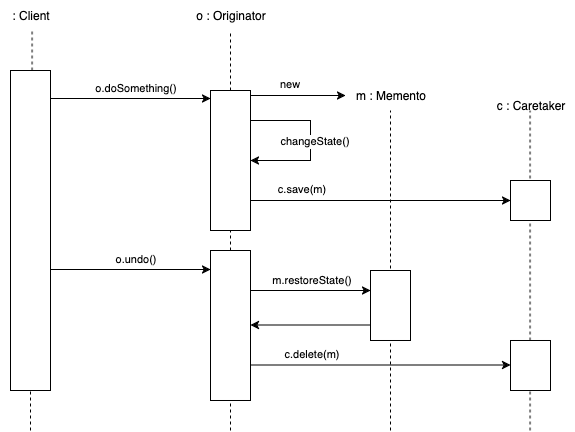
\includegraphics[width=1\linewidth]{assets/pattern/memento/memento-sequence.drawio.png}
    \caption{Sequence Diagram del pattern Memento (classico)}
\end{figure}

Il pattern permette di preservare i confini tracciati da un corretto incapsulamento, sebbene abbia un certo costo (soprattutto in termini di memoria, ma anche di gestione).

\newpage